\documentclass[10pt]{article}
\usepackage[english]{babel}
\usepackage{geometry}[scale=0.88]
\usepackage{amsmath,amssymb,graphicx,alltt,theorem}
\usepackage{float}
\usepackage{cite}
\usepackage{listings}
\usepackage{xcolor}
\usepackage{abstract}
\usepackage[colorlinks, linkcolor=red, anchorcolor=blue, citecolor=green]{hyperref}

 \lstset{
 columns=fixed, 
 basicstyle=\footnotesize\ttfamily\scriptsize,   
 numberstyle=\tiny\color{gray},                      
 frame=none,                                        
%  backgroundcolor=\color[RGB]{245,245,244},          
 keywordstyle=\color[RGB]{40,40,255},               
 numberstyle=\footnotesize\color{darkgray},           
 commentstyle=\ttfamily\color[RGB]{0,96,96},              
 stringstyle=\ttfamily\color[RGB]{128,0,0}, 
 showstringspaces=false,      
 xleftmargin=0.03\textwidth, xrightmargin=0.05\textwidth                       
}

\setlength{\parindent}{0pt}
\linespread{1.2}


%%%%%%%%%% Start TeXmacs macros
% \newcommand{\assign}{:=}
% \newcommand{\tmaffiliation}[1]{\\ #1}
% \newcommand{\tmem}[1]{{\em #1\/}}
% \newcommand{\tmop}[1]{\ensuremath{\operatorname{#1}}}
% \newcommand{\tmsamp}[1]{\textsf{#1}}
% \newcommand{\tmstrong}[1]{\textbf{#1}}
% \newcommand{\tmtextit}[1]{\text{{\itshape{#1}}}}
% \newcommand{\tmverbatim}[1]{\text{{\ttfamily{#1}}}}
\newenvironment{tmcode}[1][]{\begin{alltt} }{\end{alltt}}
{\theorembodyfont{\rmfamily}\newtheorem{remark}{Remark}}
%%%%%%%%%% End TeXmacs macros

% \newcommand{\X}{\mathbf{X}}
% \newcommand{\A}{\mathbf{A}}
% \newcommand{\C}{\mathbf{C}}
% \newcommand{\tmb}{\mathbf{b}}
% \newcommand{\0}{\textbf{0}}
% \newcommand{\x}{\mathbf{x}}
% \newcommand{\y}{\mathbf{y}}
% \newcommand{\bs}{\mathbf{S}}
% \newcommand{\tmc}{\mathbf{c}}
% \newcommand{\z}{\ensuremath{\mathbf{z}}}
% \newcommand{\I}{\mathbf{I}}
% \newcommand{\fa}{\mathcal{A}}
% \newcommand{\tmr}{\mathbf{r}}
% \newcommand{\p}{\mathbf{p}}
% \newcommand{\M}{\mathbf{M}}
% \newcommand{\tmd}{\ensuremath{\mathbf{d}}}
% \newcommand{\R}{\mathbf{R}}
% \newcommand{\m}{\ensuremath{\mathbf{m}}}
% \newcommand{\tmu}{\mathbf{u}}
% \newcommand{\s}{\mathbf{s}}
% \newcommand{\e}{\mathbf{e}}
% \newcommand{\tma}{\mathbf{a}}

% \newcommand{\hdsdp}{{\texttt{HDSDP}}}
% \newcommand{\dsdp}{{\texttt{DSDP}}}
% \newcommand{\dsdpbenson}{{\texttt{DSDP5.8}}}

\usepackage{enumitem}
\usepackage{xcolor}

\begin{document}

\title{HDSDP: Software for Semidefinite Programming}

\author{Wenzhi Gao\thanks{gwz@163.shufe.edu.cn} \quad Dongdong Ge\thanks{ge.dongdong@mail.shufe.edu.cn} \quad Yinyu Ye\thanks{yyye@stanford.edu}}
\maketitle

\begin{abstract}
  HDSDP is a numerical software solving the semidefinite
  programming problems. The main framework of {{\texttt{HDSDP}}} resembles the dual-scaling
  interior point solver {{\texttt{DSDP}}}{\cite{benson2008algorithm}} and several new
  features, especially a dual method based on the simplified homogeneous
  self-dual embedding, have been implemented. The embedding enhances stability of dual method 
  and several new heuristics and computational techniques are designed to accelerate its
  convergence. HDSDP aims to show how dual-scaling algorithms benefit from the
  self-dual embedding and it is developed in parallel to {{{\texttt{DSDP5.8}}}}.
  Numerical experiments over several classical benchmark datasets exhibit its
  robustness and efficiency, and particularly its advantages on XXX structure problems.
\end{abstract}
\section{Introduction}

Semidefinite programming (SDP) is a mathematical programming problem defined
by
\begin{eqnarray}
  \min_{\mathbf{X}} & \left\langle \mathbf{C}, \mathbf{X} \right\rangle & \nonumber \\
  \text{subject to} & \mathcal{A} \mathbf{X} = \mathbf{b} & \\ 
  & \mathbf{X} \in \mathbb{S}_+^n, & \nonumber
\end{eqnarray}
where we study linear optimization subject to affine constraints over the cone of
positive-semidefinite matrices. Due to its extensive modeling capability, SDP
has been employed in various communities including combinatorial
optimization{\cite{goemans1995improved, laurent2005semidefinite}},
dynamic systems {\cite{vandenberghe1996semidefinite}}, sums of squares
optimization{\cite{laurent2009sums}}, quantum
information{\cite{hayashi2016quantum}}, and distance geometry
{\cite{biswas2004semidefinite, so2007theory}}. We refer the interested
readers to {\cite{wolkowicz2005semidefinite}} for a more comprehensive review
of SDP applications. \\

While SDP proves useful in many applications, a fundamental issue is how to
numerically solve them. Theoretically, SDP is a convex conic problem which
admits efficient polynomial-time algorithms and for general SDPs, the interior
point method (IPM) is known as a most robust and efficient approach. Since the
1990s, high-performance SDPs softwares based on the IPM have been developed,
including {{\texttt{DSDP}}} {\cite{benson2008algorithm}}, \text{{\ttfamily{COPT}}}
{\cite{copt}}, \text{{\ttfamily{Mosek}}} {\cite{aps2019mosek}}, \text{{\ttfamily{Sedumi}}}
{\cite{polik2007sedumi}}, \text{{\ttfamily{SDPT3}}} {\cite{toh2012implementation}},
\text{{\ttfamily{CSDP}}} {\cite{borchers2006csdp}} and \text{{\ttfamily{SDPA}}}
{\cite{yamashita2012latest}}. While most SDP codes implement the IPM, there also exist
a number of successful attempts adopting other algorithms including
{\cite{kocvara2006pensdp, kwasniewiczimplementation, yang2015sdpnal}}
and a list of such SDP software is available from {\cite{majumdar2020recent}}.\\

SDP solvers based on different IPM variants enjoy nice convergence behavior
both theoretically and practically. Most SDP solvers implement a
path-following primal-dual approach either using infeasible start
{\cite{potra1998superlinearly}} or the homogeneous self-dual embedding
{\cite{potra1998homogeneous}} with {{\texttt{DSDP}}} being an exception.
{{\texttt{DSDP}}} implements a dual IPM method based on the potential reduction framework 
proposed in {\cite{benson1999mixed}}.
Since the initial release {\cite{benson2000solving}}, {{\texttt{DSDP}}} has
gone a long way through several major updates and evolved into an
efficient and robust solver for general SDPs {\cite{benson2008algorithm}}.
To further enhance the efficiency and robustness of {{\texttt{DSDP}}}, we make
another extension by incorporating the well-known homogeneous self-dual (HSD)
embedding into the dual algorithm. This new implementation, named
{{\texttt{HDSDP}}}, is presented in this manuscript.\\

The rest of the manuscript is organized as follows. \textbf{Section \ref{sec2}} 
describes the SDP formulation of interest and basic notations.
{\textbf{Section \ref{sec3}} reviews the dual-scaling algorithm for SDP
and describes how to combine it with the simplified HSD embedding. In {\textbf{Section
\ref{sec4}} and \textbf{\ref{sec5}}, we introduce the practical aspects for {{\texttt{HDSDP}}}. 
Last we present the computational results of various SDP problems.

\section{Formulation and Notations} \label{sec2}

{{\texttt{HDSDP}}} is interested in the standard form primal SDP and its dual

{\center{$\begin{array}{lccl}
  (P) & \min_{\mathbf{X}}  & \left\langle \mathbf{C}, \mathbf{X} \right\rangle & \\
  & \text{subject to} & \left\langle \mathbf{A}_i, \mathbf{X} \right\rangle = \mathbf{b}, & i = 1,
  \ldots, m\\
  &  & \mathbf{X} \in \mathbb{S}_+^n & 
\end{array}$\qquad$\begin{array}{lcc}
  (D) & \max_{\mathbf{y}, \mathbf{S}} & \mathbf{b}^{\top} \mathbf{y}\\
  & \text{subject to} & \sum_{i = 1}^m \mathbf{A}_i y_i + \mathbf{S} = \mathbf{C}\\
  &  & \mathbf{S} \in \mathbb{S}_+^n,
\end{array}$}}\\

where the problem data $\{\mathbf{A}_i\}, \mathbf{C}$ are $n \times n$ symmetric matrices
($\mathbb{S}^n$) and $\mathbf{b} \in \mathbb{R}^m$ is a real vector. Matrix inner
product $\langle \cdot, \cdot \rangle$ is defined by $\left\langle \mathbf{A}, \mathbf{X} \right\rangle := \sum_{k, l}
c_{i j} x_{i j}$ and $\mathbb{S}_+^n$ denotes the cone of positive
semidefinite matrices. For brevity we use $\mathbf{X} \succeq \textbf{0}$ to denote the
relation $\mathbf{X} \in \mathbb{S}_+^n$ and the linear map $\mathcal{A} : \mathbb{S}^n
\rightarrow \mathbb{R}^m$ and its adjoint $\mathcal{A}^{\ast} : \mathbb{R}^m
\rightarrow \mathbb{S}^n$ are respectively defined by $\mathcal{A} \mathbf{X} := \left(
\left\langle \mathbf{A}, \mathbf{X}_1 \right\rangle, \ldots, \left\langle \mathbf{A}_m, \mathbf{X}_m
\right\rangle \right)^{\top}$ and $\mathcal{A}^{\ast} \mathbf{y} := \sum_{i = 1}^m \mathbf{A}_i
y_i$. $\left\| \mathbf{A} \right\|_F := \sqrt{\sum_{i j} a_{i j}^2}$ denotes
matrix Frobenius norm. With the above notations, we rewrite the primal and
dual problems by

{\center{$\begin{array}{lccl}
  (P) & \min_{\mathbf{X}}  & \left\langle \mathbf{C}, \mathbf{X} \right\rangle & \\
  & \text{subject to} & \mathcal{A} \mathbf{X} = \mathbf{b}, & i = 1, \ldots, m\\
  &  & \mathbf{X} \succeq \textbf{0} & 
\end{array}$\qquad$\begin{array}{lcc}
  (D) & \max_{\mathbf{y}, \mathbf{S}} & \mathbf{b}^{\top} \mathbf{y}\\
  & \text{subject to} & \mathcal{A}^{\ast} \mathbf{y} + \mathbf{S} = \mathbf{C}\\
  &  & \mathbf{S} \succeq \textbf{0} .
\end{array}$}}\\

and the feasible regions for $(P)$ and $(D)$ are respectively
$\mathcal{F} (P) := \left\{ \mathbf{X} : \mathcal{A} \mathbf{X} = \mathbf{b}, \mathbf{X} \succeq \textbf{0} \right\}$
and $\mathcal{F} (D) := \left\{ \left( \mathbf{y}, \mathbf{S} \right) : \mathcal{A}^{\ast} \mathbf{y} +
\mathbf{S} = \mathbf{C}, \mathbf{S} \succeq \textbf{0} \right\}$. Any $\mathbf{X} \in \mathcal{F} (P)$ is called primal
feasible and $\left( \mathbf{y}, \mathbf{S} \right) \in \mathcal{F} (D)$ is dual feasible.
The interior of the feasible regions are denoted by $\mathcal{F}^0 (P),
\mathcal{F}^0 (D)$ and any point in $\mathcal{F}^0$ is called an interior
point solution. 

\begin{remark}
  Although in this manuscript we focus on the SDP of single-block for ease of
  exposition, a natural generalization to multi-block SDPs applies rather
  straightforward.
\end{remark}

{{\texttt{HDSDP}}} implements a dual method that solves both
({{\em P\/}}) and ({{\em D\/}}) through the simplified HSD and in the next
section we get down to the underlying theoretical details.


\section{Homogeneous Dual Scaling Algorithm }\label{sec3}

In this section we review the dual-scaling algorithm in
{{\texttt{DSDP}}} and its interpretations through Newton's method. Then
we show how the simplified HSD embedding applies to the dual method leveraging 
this interpretation.

\subsection{Dual-scaling Algorithm}

The dual-scaling algorithm for SDP is initially proposed in
{\cite{benson1999mixed}} and works under three conditions. {\textbf{1)}} the
 data $\left\{ \mathbf{A}_i \right\}$ are linearly independent.
{\textbf{2)}} ({{\em P\/}}) and ({{\em D\/}}) both admit interior point
solution. {\textbf{3)}} an interior dual feasible solution $\left( \mathbf{y}^0,
\mathbf{S}^0 \right) \in \mathcal{F}^0 (D)$ is known. The first two conditions imply
strong duality and the existence of a primal-dual optimal pair $\left(
\mathbf{X}^{\ast}, \mathbf{y}^{\ast}, \mathbf{S}^{\ast} \right)$ satisfying complementarity condition
$\left\langle \mathbf{X}^{\ast}, \mathbf{S}^{\ast} \right\rangle = 0$ and $\mathbf{X} \mathbf{S} = \textbf{0}$.
Also, the central path $\mathcal{C} (\mu) :=
\left\{ \left( \mathbf{X}, \mathbf{y}, \mathbf{S} \right) \in \mathcal{F}^0 (P) \times \mathcal{F}^0
(D) : \mathbf{X} \mathbf{S} = \mu \mathbf{I} \right\}$ is guaranteed to exist,  which serves as the foundation of the
path-following IPMs. Given barrier parameter $\mu$, by the last condition, 
dual-scaling starts from a dual-feasible solution
$\left( \mathbf{y}, \mathbf{S} \right)$ and takes Newton's step towards $\mathcal{A} \mathbf{X} = \mathbf{b},
\mathcal{A}^{\ast} \mathbf{y} + \mathbf{S} = \mathbf{C}$ and $\mathbf{X} \mathbf{S} = \mu \mathbf{I}$ by solving
\begin{eqnarray}\label{dsdpnewton}
  \mathcal{A} \left( \mathbf{X} + \Delta \mathbf{X} \right) & = & \mathbf{b} \nonumber \\
  \mathcal{A}^{\ast} \Delta \mathbf{y} + \Delta \mathbf{S} & = & \textbf{0} \\
  \mu \mathbf{S}^{- 1} \Delta \mathbf{S} \mathbf{S}^{- 1} + \Delta \mathbf{X} & = & \mu \mathbf{S}^{- 1} - \mathbf{X} \nonumber, 
\end{eqnarray}
where the last relation linearizes $\mathbf{X} = \mu \mathbf{S}^{- 1}$ instead of $\mathbf{X} \mathbf{S} =
\mu \mathbf{I}$ and $\mathbf{S}^{- 1}$ is called a scaling matrix. 
By carefully driving $\mu$ to 0, dual-scaling eliminates infeasibility, approaches optimality, and finally solves the problem.

One feature of dual-scaling is that $\mathbf{X}$ and $\Delta \mathbf{X}$
vanish in the Schur complement system of \eqref{dsdpnewton}

\begin{eqnarray} \label{dsdpM}
	\left(\begin{array}{ccc}
     \left\langle \mathbf{A}_1, \mathbf{S}^{- 1} \mathbf{A}_1 \mathbf{S}^{- 1} \right\rangle & \cdots &
     \left\langle \mathbf{A}_1, \mathbf{S}^{- 1} \mathbf{A}_m \mathbf{S}^{- 1} \right\rangle\\
     \vdots & \ddots & \vdots\\
     \left\langle \mathbf{A}_m, \mathbf{S}^{- 1} \mathbf{A}_1 \mathbf{S}^{- 1} \right\rangle & \cdots &
     \left\langle \mathbf{A}_m, \mathbf{S}^{- 1} \mathbf{A}_m \mathbf{S}^{- 1} \right\rangle
   \end{array}\right) \Delta \mathbf{y} = \frac{1}{\mu} \mathbf{b} - \mathcal{A} \mathbf{S}^{- 1}
\end{eqnarray}\\
and the dual algorithm thereby avoids explicit reference to the primal
variable $\mathbf{X}$. For brevity we sometimes denote the left-hand side matrix in \eqref{dsdpM} by $\mathbf{M}$.
When $\left\{ \mathbf{A}_i \right\}, \mathbf{C}$ are sparse, the dual variable $\mathbf{S} = \mathbf{C}
-\mathcal{A}^{\ast} \mathbf{y}$ inherits the sparsity pattern from the data and it is
therefore cheaper to iterate in the dual space to exploit sparsity.
Another desirable feature of dual-scaling is the availablity of primal
solution by solving a projection subproblem at the end of the algorithm \cite{benson2008algorithm}. The
above properties characterize the behavior of dual-scaling.\\

However, the nice theoretical properties of the dual method is not free. 
First, an initial dual feasible solution is needed but obtaining such a
solution is often as difficult as solving the original problem. Second, due to
a lack of information from the primal space, the dual-scaling has to be
property guided to avoid deviating too far away from the central path. Last,
dual-scaling linearizes the highly nonlinear relation $\mathbf{X} = \mu \mathbf{S}^{- 1}$ and
this imposes strict constraint on the damping factor towards the Newton's
direction. To overcome the aforementioned difficulties, {{\texttt{DSDP}}}
introduces slack variables with big-$M$ penalty to ensure nonempty interior
and a trivial dual feasible solution. Moreover, a potential function is introduced 
to guide the dual iterations. These attempts works
well in practice and makes {{\texttt{DSDP}}} an efficient general SDP solver.
For a complete description of the theoretical aspects of {{\texttt{DSDP}}} and
its delicate implementation, we refer the interested readers to
{\cite{benson2000solving, benson2008algorithm}}\\

Although {{\texttt{DSDP}}} proves efficient in real practice, the big-$M$
methods requires prior estimation of the optimal solution to retain optimality. 
Also, a large penalty might lead to numerical difficulties and
misclassification of infeasible problems when the problem is ill-conditioned. 
It is natural to ask if there exists an alternative to
big-$M$ method to address these issues and in this work, we propose to
leverage the well-known HSD embedding.

\subsection{Homogeneous Dual-scaling Algorithm}

In this section, we introduce the theoretical idea behind {{\texttt{HDSDP}}}.
HSD embedding is a skew symmetric system whose non-trivial interior point
solution certificates primal-dual feasibility. \{hdsdp} adopts the simplified
HSD embedding {\cite{xu1996simplified}} and its extension to SDP
{\cite{potra1998homogeneous}}.\\

{\textbf{HSD embedding for SDP}}
\begin{eqnarray}
  \mathcal{A} \mathbf{X} - \mathbf{b} \tau & = & \textbf{0} \nonumber\\
  - \mathcal{A}^{\ast} \mathbf{y} + \mathbf{C} \tau - \mathbf{S} & = & \textbf{0}  \\
  \mathbf{b}^{\top} \mathbf{y} - \left\langle \mathbf{C}, \mathbf{X} \right\rangle - \kappa & = & 0 \nonumber\\
  \mathbf{X}, \mathbf{S} \succeq 0, &  & \kappa, \tau \geq 0 \nonumber,
\end{eqnarray}
where $\kappa, \tau \geq 0$ are homogenizing variables for infeasibility
detection. Given parameter $\mu$, we similarly define the central path
\begin{eqnarray}
  \mathcal{A} \mathbf{X} - \mathbf{b} \tau & = & \textbf{0} \nonumber \\
  - \mathcal{A}^{\ast} \mathbf{y} + \mathbf{C} \tau - \mathbf{S} & = & \textbf{0} \nonumber \\
  \mathbf{b}^{\top} \mathbf{y} - \left\langle \mathbf{C}, \mathbf{X} \right\rangle - \kappa & = & 0 \nonumber \\
  \mathbf{X} \mathbf{S} = \mu \mathbf{I}, &  & \kappa \tau = \mu \label{hdsdpcompl} \\
  \mathbf{X}, \mathbf{S} \succeq 0, &  & \kappa, \tau \geq 0. \nonumber
\end{eqnarray}
Here $\left( \mathbf{y}, \mathbf{S}, \tau \right)$ are jointly considered as dual variables.
Given a dual point $\left( \mathbf{y}, \mathbf{S}, \tau \right)$ such that $- \mathcal{A}^{\ast} \mathbf{y} +
\mathbf{C} \tau - \mathbf{S} = \mathbf{R}$, {{\texttt{HDSDP}}} chooses a damping factor $\gamma \in
(0, 1]$ and takes Newton's step towards
\begin{eqnarray*}
  \mathcal{A} \left( \mathbf{X} + \Delta \mathbf{X} \right) - \mathbf{b} (\tau + \Delta \tau) & = & \textbf{0}\\
  -\mathcal{A}^{\ast} \left( \mathbf{y} + \Delta \mathbf{y} \right) + \mathbf{C} (\tau + \Delta \tau)
  - \left( \mathbf{S} + \Delta \mathbf{S} \right) & = & - \gamma \mathbf{R}\\
  \mu \mathbf{S}^{- 1} \Delta \mathbf{S} \mathbf{S}^{- 1} + \Delta \mathbf{X} & = & \mu \mathbf{S}^{- 1} - \mathbf{X},\\
  \mu \tau^{- 2} \Delta \tau + \Delta \kappa & = & \mu \tau^{- 1} - \kappa,
\end{eqnarray*}
where, as in {{\texttt{DSDP}}}, we modify \eqref{hdsdpcompl} and linearize $\mathbf{X} = \mu \mathbf{S}^{- 1}$ and $\kappa
= \mu \tau^{- 1}$. We note that the damping factor can be chosen after the
directions are computed and for simplicity we set $\gamma = 0$. Then the
Newton's direction $\left( \Delta \mathbf{y}, \Delta \tau \right)$ is computed through
the following Schur complement.

\begin{eqnarray}
  &  & \left(\begin{array}{cc}
    \mu \mathbf{M} & - \mathbf{b} - \mu \mathcal{A} \mathbf{S}^{- 1} \mathbf{C} \mathbf{S}^{- 1}\\
    - \mathbf{b} + \mu \mathcal{A} \mathbf{S}^{- 1} \mathbf{C} \mathbf{S}^{- 1} & - \mu \left(
    \left\langle \mathbf{C}, \mathbf{S}^{- 1} \mathbf{C} \mathbf{S}^{- 1} \right\rangle + \tau^{- 2} \right)
  \end{array}\right) \left(\begin{array}{c}
    \Delta \mathbf{y}\\
    \Delta \tau
  \end{array}\right)\\ \nonumber
  & = & \left(\begin{array}{c}
    \mathbf{b} \tau\\
    \mathbf{b}^{\top} \mathbf{y} - \mu \tau^{- 1}
  \end{array}\right) - \mu \left(\begin{array}{c}
    \mathcal{A} \mathbf{S}^{- 1}\\
    \left\langle \mathbf{C}, \mathbf{S}^{- 1} \right\rangle
  \end{array}\right) + \mu \left(\begin{array}{c}
    \mathcal{A} \mathbf{S}^{- 1} \mathbf{R} \mathbf{S}^{- 1}\\
    \left\langle \mathbf{C}, \mathbf{S}^{- 1} \mathbf{R} \mathbf{S}^{- 1} \right\rangle
  \end{array}\right) \\ \nonumber
\end{eqnarray}

In practice, {{\texttt{HDSDP}}} solves $\Delta \mathbf{y}_1 := \mathbf{M}^{- 1} \mathbf{b},
\Delta \mathbf{y}_2 := \mathbf{M}^{- 1} \mathcal{A} \mathbf{S}^{- 1}, \Delta \mathbf{y}_3 := \mathbf{M}^{- 1} \mathcal{A}
\mathbf{S}^{- 1} \mathbf{R} \mathbf{S}^{- 1}, \Delta \mathbf{y}_4 = \mathbf{M}^{- 1} \mathcal{A} \mathbf{S}^{- 1} \mathbf{C} \mathbf{S}^{-
1}$, plugs $\Delta \mathbf{y} = \frac{\tau + \Delta \tau}{\mu} \Delta \mathbf{y}_1 - \Delta
\mathbf{y}_2 + \Delta \mathbf{y}_3 + \Delta \mathbf{y}_4 \Delta \tau$ into the second equation to
solve for $\Delta \tau$ and finally assembles $\Delta \mathbf{y}$ using $\tau, \Delta
\tau$ and $\mu$. With the above relations, $\mathbf{X} (\mu) := \mu \mathbf{S}^{- 1}
\left( \mathbf{S} - \mathbf{R} +\mathcal{A}^{\ast} \Delta \mathbf{y} - \mathbf{C} \Delta \tau \right) \mathbf{S}^{-
1}$ satisfies $\mathcal{A} \mathbf{X} (\mu) - \mathbf{b} (\tau + \Delta \tau) = \textbf{0}$ and $\mathbf{X} (\mu)
\succeq \textbf{0}$ iff. $-\mathcal{A}^{\ast} \left( \mathbf{y} - \Delta \mathbf{y} \right) + \mathbf{C} (\tau
- \Delta \tau) - 2 \mathbf{R} \succeq \textbf{0}$. When $-\mathcal{A}^{\ast} \left( \mathbf{y} -
\Delta \mathbf{y} \right) + \mathbf{C} (\tau - \Delta \tau) - 2 \mathbf{R}$ is positive definite, an
objective bound follows by
\begin{eqnarray*}
  \bar{z} & = & \left\langle \mathbf{C} \tau, \mathbf{X} (\mu) \right\rangle\\
  & = & \left\langle \mathbf{R} + \mathbf{S} + \mathcal{A}^{\ast} \mathbf{y}, \mu \mathbf{S}^{- 1} \left( \mathbf{S} - \mathbf{R}
  +\mathcal{A}^{\ast} \Delta \mathbf{y} - \mathbf{C} \Delta \tau \right) \mathbf{S}^{- 1}
  \right\rangle\\
  & = & (\tau + \Delta \tau) \mathbf{b}^{\top} \mathbf{y} + n \mu + \left( \mathcal{A} \mathbf{S}^{- 1} +
  \mathcal{A} \mathbf{S}^{- 1} \mathbf{R} \mathbf{S}^{- 1} \right)^{\top} \Delta \mathbf{y} + \mu \left(
  \left\langle \mathbf{C}, \mathbf{S}^{- 1} \right\rangle + \left\langle \mathbf{C}, \mathbf{S}^{- 1} \mathbf{C}
  \mathbf{S}^{- 1} \right\rangle \right) \Delta \tau
\end{eqnarray*}
and dividing both sides by $\tau$. Alternatively {{\texttt{HDSDP}}} extracts a
bound from the projection problem
\begin{eqnarray*}
  \min_{\mathbf{X}} & \left\| \mathbf{S}^{1 / 2} \mathbf{X} \mathbf{S}^{1 / 2} - \mu \mathbf{I} \right\|_F^2 & \\
  \text{subject to} & \mathcal{A} \mathbf{X} = \mathbf{b} \tau, & 
\end{eqnarray*}
whose optimal solution is $\mathbf{X}' (\mu) := \mu \mathbf{S}^{- 1} \left( \mathbf{C} \tau -
\mathcal{A}^{\ast} \left( \mathbf{y} - \Delta' \mathbf{y} \right) - \mathbf{R} \right) \mathbf{S}^{- 1}$, where
$\Delta \mathbf{y}' = \frac{\tau}{\mu} \Delta \mathbf{y}_1 - \Delta \mathbf{y}_2$ and
\[ z' = \left\langle \mathbf{C} \tau, \mathbf{X}' (\mu) \right\rangle = \mu \left\{
   \left\langle \mathbf{R}, \mathbf{S}^{- 1} \right\rangle + \left( \mathcal{A} \mathbf{S}^{- 1} \mathbf{R}_{\mathbf{y}}
   \mathbf{S}^{- 1} + \mathcal{A} \mathbf{S}^{- 1} \right)^{\top} \Delta' \mathbf{y} + n \right\} + \tau
   \mathbf{b}^{\top} \mathbf{y} . \]
In practice, when the explicit solution $\mathbf{X} (\mu)$ or $\mathbf{X}' (\mu)$ is needed,
we can decompose $\mathbf{S}$ and solve two sets of linear systems to obtain them.\\

One major computationally intensive part in {{\texttt{HDSDP}}} is the setup of
the Schur complement matrix $\mathbf{M}$. Since the objective $\mathbf{C}$ often does not
enjoy the same structure as $\left\{ \mathbf{A}_i \right\}$, the additional cost from
$\mathcal{A} \mathbf{S}^{- 1} \mathbf{C} \mathbf{S}^{- 1}$ and $\left\langle \mathbf{C}, \mathbf{S}^{- 1} \mathbf{C} \mathbf{S}^{- 1}
\right\rangle$ calls for more efficient techniques to set up $\mathbf{M}$. In
{{\texttt{HDSDP}}}, a permutation $\sigma (m)$ of the rows of $\mathbf{M}$ is
generated heuristically and $\mathbf{M}$ is then set up using one of the following five
techniques row-by-row.

\[ \left(\begin{array}{ccc}
     \left\langle \mathbf{A}_{\sigma (1)}, \mathbf{S}^{- 1} \mathbf{A}_{\sigma (1)} \mathbf{S}^{- 1}
     \right\rangle & \cdots & \left\langle \mathbf{A}_{\sigma (1)}, \mathbf{S}^{- 1}
     \mathbf{A}_{\sigma (m)} \mathbf{S}^{- 1} \right\rangle\\
     & \ddots & \vdots\\
     &  & \left\langle \mathbf{A}_{\sigma (m)}, \mathbf{S}^{- 1} \mathbf{A}_{\sigma (m)} \mathbf{S}^{- 1}
     \right\rangle
   \end{array}\right) \]\\
   
Technique {\textbf{M1}} and {\textbf{M2}} are inherited from
{{\texttt{DSDP}}}. They exploit the low-rank structure of the problem data and
an eigen-decomposition of the problem data
\[ \mathbf{A}_i = \sum_{r = 1}^{\ensuremath{\operatorname{rank}} \left( \mathbf{A}_i \right)} \lambda_{i r}
   \mathbf{a}_{i, r} \mathbf{a}^{\top}_{i, r} \]
has to be computed at the beginning of the algorithm.\\

\begin{center}
\fbox{	\begin{minipage}{0.8\textwidth}
		{\textbf{Technique M1}}
\begin{enumerate}
  \item {\textbf{Setup}} $\mathbf{B}_{\sigma (i)} = \sum_{r =
  1}^{\ensuremath{\operatorname{rank}} \left( \mathbf{A}_{\sigma (i)} \right)} \lambda_r \left( \mathbf{S}^{- 1}
  \mathbf{a}_{\sigma (i), r} \right) \left( \mathbf{S}^{- 1} \mathbf{a}_{\sigma (i), r}
  \right)^{\top}$.
  
  \item {\textbf{Compute}} $M_{\sigma (i) \sigma (j)} = \left\langle
  \mathbf{B}_{\sigma (i)}, \mathbf{A}_{\sigma (j)} \right\rangle, \forall j \geq i$.
\end{enumerate}
{\textbf{Technique M2}}
\begin{enumerate}
  \item {\textbf{Setup}} $\mathbf{S}^{- 1} \mathbf{a}_{\sigma (i), r}, r = 1, \ldots,
  r_{\sigma (i)}$.
  \item {\textbf{Compute}} $M_{\sigma (i) \sigma (j)} = \sum_{r =
  1}^{\ensuremath{\operatorname{rank}} \left( \mathbf{A}_{\sigma (i)} \right)} \left( \mathbf{S}^{- 1}
  \mathbf{a}_{\sigma (i), r} \right)^{\top} \mathbf{A}_{\sigma (j)} \left( \mathbf{S}^{- 1}
  \mathbf{a}_{\sigma (i), r} \right)$.
\end{enumerate}
\end{minipage}} 
\end{center}
Technique {\textbf{M3}}, {\textbf{M4}} and {\textbf{M5}} exploit the sparsity of the constraints and needs evaluation of $\mathbf{S}^{-1}$.
{\cite{fujisawa1997exploiting}}.
\begin{center}
	\fbox{\begin{minipage}{0.8\textwidth}
{\textbf{Technique M3}}
\begin{enumerate}
  \item {\textbf{Setup}} $\mathbf{B}_{\sigma (i)} = \mathbf{S}^{- 1} \mathbf{A}_{\sigma
  (i)} \mathbf{S}^{- 1}$.
  
  \item {\textbf{Compute}} $M_{\sigma (i) \sigma (j)} = \left\langle
  \mathbf{B}_{\sigma (i)}, \mathbf{A}_{\sigma (j)} \right\rangle, \forall j \geq i$.
\end{enumerate}
{\textbf{Technique M4}}
\begin{enumerate}
  \item {\textbf{Setup}} $\mathbf{B}_{\sigma (i)} = \mathbf{S}^{- 1} \mathbf{A}_{\sigma
  (i)}$.
  
  \item {\textbf{Compute}} $M_{\sigma (i) \sigma (j)} = \left\langle
  \mathbf{B}_{\sigma (i)} \mathbf{S}^{- 1}, \mathbf{A}_{\sigma (j)} \right\rangle, \forall j
  \geq i$.
\end{enumerate}
{\textbf{Technique M5}}
\begin{enumerate}
  \item {\textbf{Compute}} $M_{\sigma (i) \sigma (j)} = \left\langle \mathbf{S}^{-
  1} \mathbf{A}_{\sigma (i)} \mathbf{S}^{- 1}, \mathbf{A}_{\sigma (j)} \right\rangle, \forall j \geq
  i$ directly.\
\end{enumerate}
\end{minipage}}
\end{center}\


At the beginning of the algorithm, {{\texttt{HDSDP}}} estimates the
number of flops using each technique and each row of $\mathbf{M}$ is associated with the cheapest
technique to minimize the overall computation cost. This is a major
improvement over {{\texttt{DSDP5.8}}} in the computational aspect and 
we leave the details to the later sections. \\

After setting up $\mathbf{M}$, conjugate gradient (CG) method is
employed to solve the linear systems. The maximum number of iterations is
chosen around $50 / m$ and is heuristically adjusted. Either the diagonal of
$\mathbf{M}$ or its Cholesky decomposition is chosen as pre-conditioner and
after a Cholesky pre-conditioner is computed, {{\texttt{HDSDP}}} reuses it for 
the consecutive solves till a heuristic determines that the current
pre-conditioner is outdated. When the algorithm approaches optimality, $\mathbf{M}$
might become ill-conditioned and {{\texttt{HDSDP}}} switches to {\textsf{LDLT}} decomposition in case Cholesky fails.\\

Using the Newton's direction, {{\texttt{HDSDP}}} computes the maximum stepsize
$$\alpha = \max \left\{ \alpha \in [0, 1] : \mathbf{S} + \alpha \Delta \mathbf{S} \succeq \textbf{0},
\tau + \alpha \Delta \tau \geq 0 \right\}$$ via a Lanczos procedure
{\cite{toh2002note}}. Then to determine a proper stepsize, one line-search
determines $\alpha_c$ such that the barrier satisfies $- \log \det \left( \mathbf{S}
+ \alpha_c \Delta \mathbf{S} \right) - \log \det (\tau + \alpha_c \Delta \tau) \leq -
\log \det \left( \mathbf{S} + \alpha_c \Delta \mathbf{S} \right) - \log \det (\tau +
\alpha_c \Delta \tau)$ and a second line-search chooses $\gamma$ such that $\mathbf{S}
+ \alpha_c \mathcal{A}^{\ast} \Delta \mathbf{y}_2 + \alpha_c \gamma \left( \mathbf{R}
-\mathcal{A}^{\ast} \Delta \mathbf{y}_3 \right) \succeq \textbf{0}$. Next a full direction
$\left( \Delta \mathbf{y}^{\gamma}, \Delta \mathbf{S}^{\gamma}, \Delta \tau^{\gamma} \right)$
is assembled from the Newton system with damping factor $\gamma$ and
a third Lanczos procedure computes $\alpha' = \max \left\{ \alpha \in [0, 1] :
\mathbf{S} + \alpha \Delta \mathbf{S}^r \succeq \textbf{0}, \tau + \alpha \Delta \tau^r \geq 0
\right\}$. Last {{\texttt{HDSDP}}} updates $\mathbf{y} \leftarrow \mathbf{y} + 0.95 \alpha'
\Delta \mathbf{y}^r$ and $\tau \leftarrow \tau + 0.95 \alpha \Delta \tau^r$. To make
further use of the Schur matrix and to maintain centrality, the
above procedure is repeated several times in an iteration. \\

In {{\texttt{HDSDP}}}, the update of the barrier parameter $\mu$ is another
critical factor. At the end of each iteration, {{\texttt{HDSDP}}} updates the
barrier parameter $\mu$ by $\left( \bar{z} - \mathbf{b}^{\top} \mathbf{y} + \theta \left\|
\mathbf{R} \right\|_F \right) / \rho n$, where $\rho$ and $\theta$ are pre-defined
parameters. Heuristics also adjust $\mu$ using  previously computed $\alpha_c, \alpha'$ and $\gamma$. \\

To get the best of the two worlds, {{\texttt{HDSDP}}} implements the same
dual-scaling algorithm as in \text{{\ttfamily{DSDP5.8}}} assuming a dual feasible solution. 
When the dual infeasibility
$\left\| \mathcal{A}^{\ast} \mathbf{y} + \mathbf{S} - \mathbf{C} \right\|_F \leq \varepsilon \tau$ and $\mu$
are sufficiently small, {{\texttt{HDSDP}}} fixes $\tau = 1$, re-starts with
$\left( \mathbf{y} / \tau, \mathbf{S} / \tau \right)$ and applies dual-scaling to guide
convergence. For the detailed implementation of dual-scaling in
\text{{\ttfamily{DSDP5.8}}} refer to {\cite{benson2008algorithm}}. To sum up,
{{\texttt{HDSDP}}} implements strategies and computational tricks tailored for
the embedding and can switch to {{\texttt{DSDP5.8}}} once a dual feasible solution is available.

\section{Initialization and Feasibility Certificate} \label{sec4}

Internally {{\texttt{HDSDP}}} deals with the following problem
\begin{eqnarray*}
  \min_{\mathbf{X}} & \left\langle \mathbf{C}, \mathbf{X} \right\rangle + \mathbf{u}^{\top} \mathbf{x}_u +
  \mathbf{l}^{\top} \mathbf{x}_l & \\
  \text{subject to} & \mathcal{A} \mathbf{X} + \mathbf{x}^u - \mathbf{x}^l = \mathbf{b} & \\
  & \mathbf{X} \succeq \textbf{0}, \mathbf{x}_u \geq \textbf{0}, \mathbf{x}_l \geq \textbf{0} & 
\end{eqnarray*}
and together with its dual, the HSD embedding is
\begin{eqnarray*}
  \mathcal{A} \mathbf{X} + \mathbf{x}^u - \mathbf{x}^l - \mathbf{b} \tau & = & \textbf{0}\\
  - \mathcal{A}^{\ast} \mathbf{y} + \mathbf{C} \tau - \mathbf{S} & = & \textbf{0}\\
  \mathbf{b}^{\top} \mathbf{y} - \left\langle \mathbf{C}, \mathbf{X} \right\rangle - \mathbf{u}^{\top} \mathbf{x}_u -
  \mathbf{l}^{\top} \mathbf{x}_l - \kappa & = & 0\\
  \mathbf{X}, \mathbf{S} \succeq 0, &  & \kappa, \tau \geq 0,
\end{eqnarray*}
where the primal problem is relaxed by two slack variables with penalty
$\textbf{{\textbf{l}}}, \mathbf{u}$ to prevent $\mathbf{y}$ going too large. Using the embedding, 
{{\texttt{HDSDP}}} needs no big-$M$ initialization
in the dual variable and starts from arbitrary $\mathbf{S} \succ \textbf{0}, \tau > 0$. By default
default $\mathbf{S}$ is initialized by a multiple of the identity matrix.

One feature of the HSD embedding is its capability to
detect infeasibility. Given infeasibility tolerance $\varepsilon_f$, {{\texttt{HDSDP}}}
classifies the problem as primal unbounded, dual infeasible if $\left\| \mathbf{R}
\right\|_F > \varepsilon_f \tau, \tau / \kappa < \varepsilon_f$ and $\mu /
\mu_0 \leq \varepsilon_f^2$. If $\mathbf{R}$ is eliminated by {{\texttt{HDSDP}}}, then
the embedding certificates dual feasibility. If $\mathbf{b}^{\top} \mathbf{y} >
\varepsilon_f^{- 1}$, then {{\texttt{HDSDP}}} begins checking if the Newton's
step $\left( \Delta \mathbf{y}, \Delta \mathbf{S} \right)$ is a dual improving ray. Once a ray is detected, the problem is classified as primal
infeasible dual unbounded.

\section{HDSDP Software}\label{sec5}

{{\texttt{HDSDP}}} is written in \text{{\ttfamily{ANSI C}}} and provides a
self-contained user interface. After the user inputs the data and invokes the
optimization routine, {{\texttt{HDSDP}}} goes through several modules
including input check, pre-solving, two-phase optimization, solution recovery
and post-solving. The modules are implemented independently and are
sequentially organized in a pipeline by {{\texttt{HDSDP}}}.

\subsection{Pre-solver}

One important feature of {{\texttt{HDSDP}}} is a special pre-solving module
 designed for SDPs. It inherits strategies from
{{\texttt{DSDP5.8}}} and adds new tricks to work jointly with the
optimization module.\\

When the pre-solver is invoked, it first goes through the problem data
$\left\{ \mathbf{A}_i \right\}$ two rounds to detect the possible low-rank structure.
The first round uses Gaussian elimination for rank-one structure and the
second round applies eigenvalue decomposition from \text{{\ttfamily{Lapack}}}. Two
exceptions are when the data matrix is too dense or sparse. If a matrix looks
too dense to be decomposed efficiently, it is skipped and marked as full-rank;
if it has very few entries, an elegant solution from {{\texttt{DSDP5.8}}} is
applied: {\textbf{1)}} a permutation gathers the non-zeros to a much smaller
dense block. {\textbf{2)}} dense eigen routines from \text{{\ttfamily{Lapack}}}
applies. {\textbf{3)}} the inverse permutation recovers the decomposition.\\

After detecting the hidden low-rank structures, the pre-solver moves on to
the analysis of the Schur matrix $\mathbf{M}$: {\textbf{1)}}. the sparsity and rank
information of the matrices are collected. {\textbf{2)}}. a permutation of
$\left\{ \mathbf{A}_i \right\}$ is generated in descending order of sparsity.
{\textbf{3)}}. for each row of $\mathbf{M}$, the flops using each of {\textbf{M1}}
to {\textbf{M5}} technique is computed and the cheapest technique is
recorded. The recorded techniques reduces the flops to set up $\mathbf{M}$ and
accelerates the convergence.\\

Last the pre-solver scales the coefficients and goes on to detect the
following structures. {\textbf{1)}}. Implied trace: constraints implying
$\ensuremath{\operatorname{tr}} \left( \mathbf{X} \right) = \theta$. {\textbf{2)}}. Implied dual bound:
constraints implying $\mathbf{l} \leq \mathbf{y} \leq \mathbf{u}$. {\textbf{3)}}. Empty
primal interior: constraints implying $\ensuremath{\operatorname{tr}} \left( \mathbf{X} \mathbf{a} \mathbf{a}^{\top}
\right) \approx 0$. {\textbf{4)}}. Empty dual interior: constraints implying
$\mathbf{A}^{\top} \mathbf{y} = \mathbf{C}$. {\textbf{5)}}. Feasibility problem. $\mathbf{C} = \textbf{0}$. For each
of the cases above the solver adjusts its internal strategies to enhance the
numerical stability and convergence.

\subsection{Two-phase Optimization}

{{\texttt{HDSDP}}} implements two phase-algorithm which integrates HSD
embedding (\text{{\ttfamily{Phase A}}}) and dual-scaling (\text{{\ttfamily{Phase B}}}). \
\text{{\ttfamily{Phase A}}} targets feasibility certificate and numerical stability,
while \text{{\ttfamily{Phase B}}} aims to efficiently drive a dual-feasible solution to
optimality using potential function.

\begin{figure}[h]
\centering
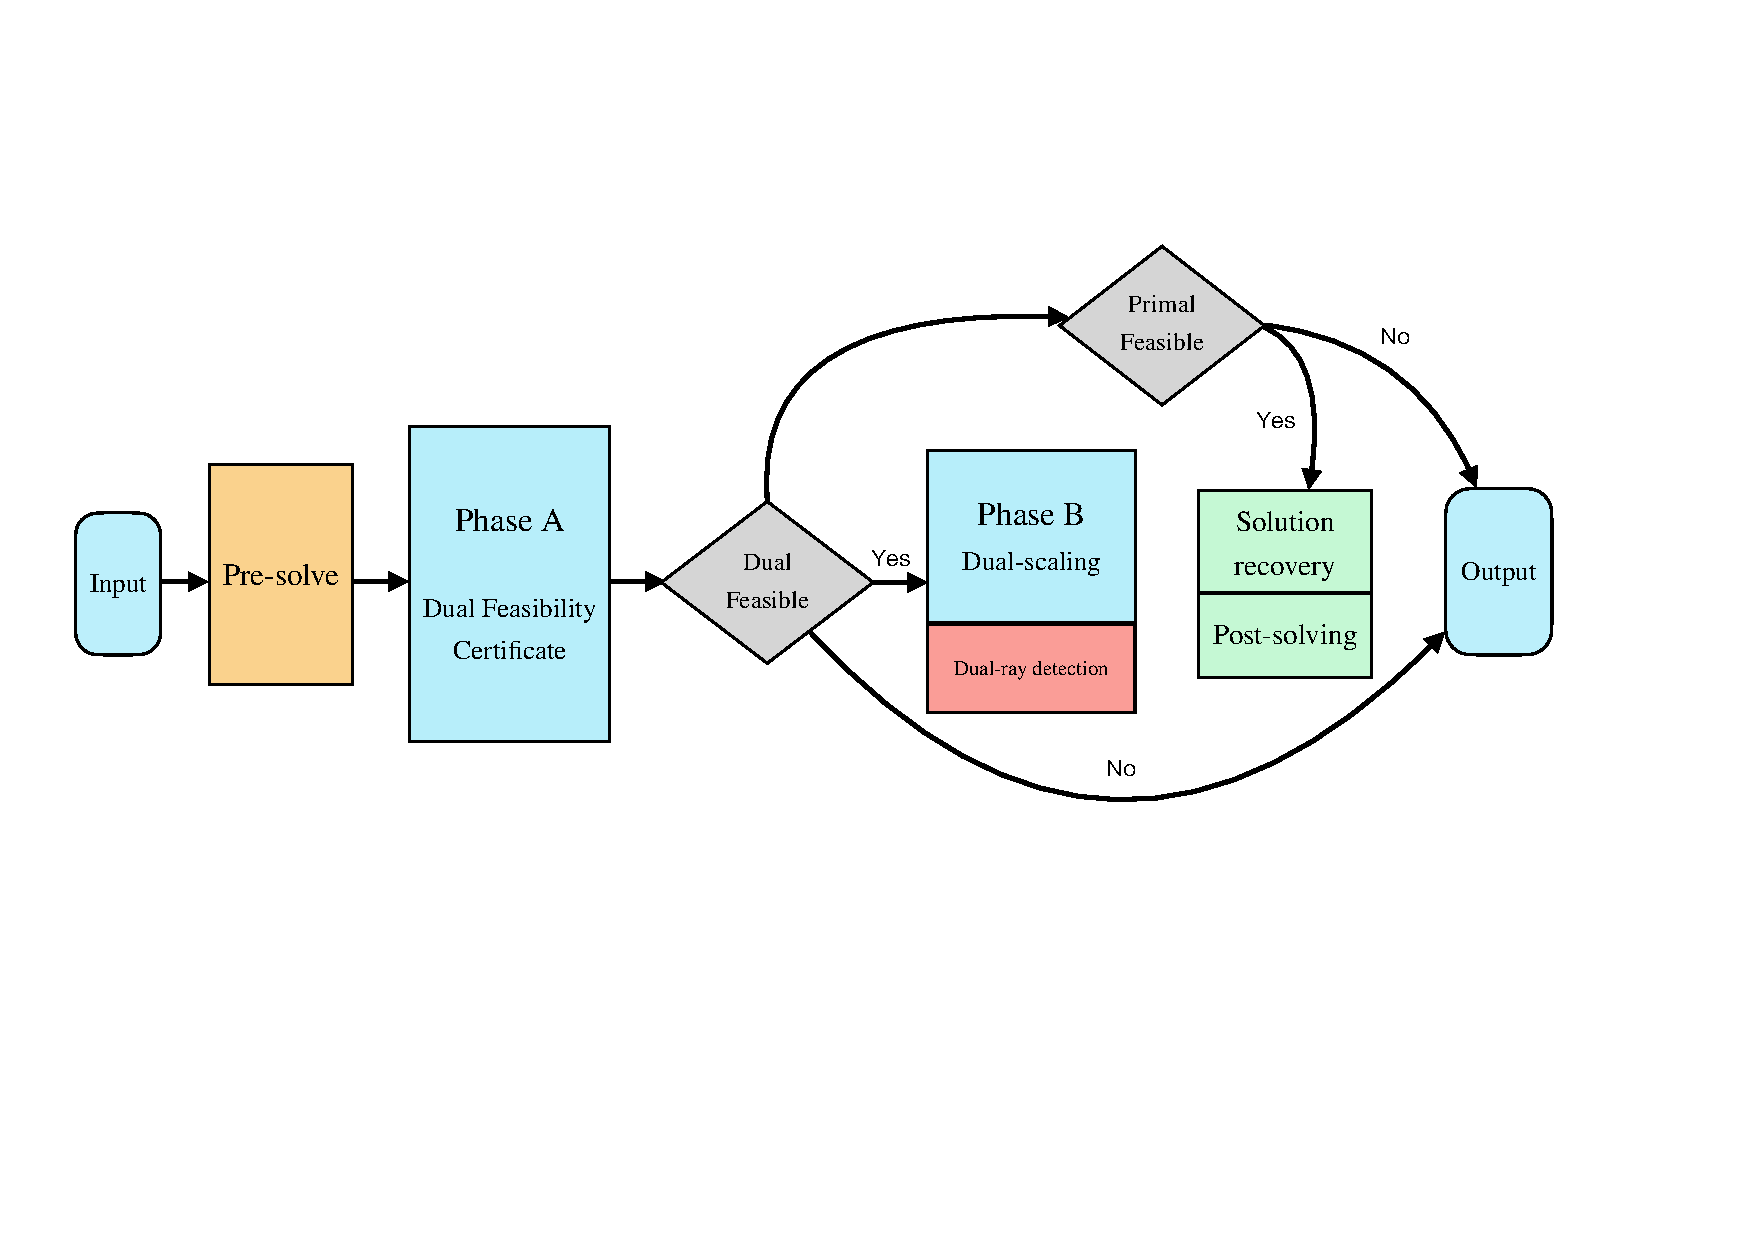
\includegraphics[scale=0.5]{fig.pdf}
  \caption{Pipeline of {{\texttt{HDSDP}}}}
\end{figure}

\

In a word, the two phases share the same backend computation routines but are
associated with different goals and strategies. {{\texttt{HDSDP}}} decides
which strategy to use based on the solution behavior.

\subsection{Iteration Monitor}

To help the users capture the progress of the solver, {{\texttt{HDSDP}}}
prints related information to the screen at different stages of optimization. 
\begin{lstlisting}
--------------------------------------------------------------------------------------
| Start presolving 
| - XXX completes in 0.001 seconds 
| - Matrix statistics ready in 0.000 seconds 
|    Schur Re-ordering: M1: 0  M2: 3000  M3: 0  M4: 1  M5: 0 
| - Special structures found 
|    tr(X) = 3.00e+03 : Bound of X fixed 
| Presolve Ends. Elapsed Time: 0.371 seconds 
--------------------------------------------------------------------------------------
\end{lstlisting}
While pre-solving, {{\texttt{HDSDP}}} prints time statistics when certain operation
is done. Specially, the row
\begin{tmcode}
      Schur Re-ordering: M1: 0  M2: 3000  M3: 0  M4: 1  M5: 0
\end{tmcode}
indicates how many times each Schur complement technique is applied and if
special SDP structures are detected, they are also printed to the screen.
\begin{tmcode}
      tr(X) = 3.00e+03 : Bound of X fixed.
\end{tmcode}
When the pre-solving ends, {{\texttt{HDSDP}}} prints matrix statistics
including type and sum of norm. Also, the solver internally adjusts its parameters
based on the collected information and display them to the user. 

\begin{lstlisting}
--------------------------------------------------------------------------------------
| Matrix statistics [Including C]: 
--------------------------------------------------------------------------------------
|     Zero |   Sparse |    Dense |   Rank-1 |      |A|    |      |b|    |      |C|     
--------------------------------------------|-----------------------------------------
|        0 |        1 |        0 |     3000 |  3.0000e+03 |  3.0000e+03 |  1.2000e+04 
--------------------------------------------------------------------------------------
| Parameter Summary: 
--------------------------------------------------------------------------------------
| Rhon [1.0, 10.0]: 5 
| Golden linesearch \{0, 1\}: 0 
| Primal relaxation penalty (0.0, inf): 1e+07 
| Time limit (0.0, inf): 15000 
| Corrector A: 4  Corrector B: 0 
--------------------------------------------------------------------------------------
| DSDP is initialized with Ry = -1.225e+05 * I                                                     
| DSDP Phase A starts. Eliminating dual infeasibility                                              
--------------------------------------------------------------------------------------
\end{lstlisting}

After pre-solving, {{\texttt{HDSDP}}} enters optimization, invokes HSD embedding (\text{{\ttfamily{Phase A}}}), and prints logs.

\begin{lstlisting}
--------------------------------------------------------------------------------------
| Iter |     pObj |     dObj |     dInf |     k/t |      mu |   step |   Pnorm |   E |
--------------------------------------------------------------------------------------
|    1 |  1.0e+05 |  0.0e+00 | 6.71e+06 | 1.0e+00 | 4.0e+04 |   0.00 | 1.0e+20 |     |
|    2 |  2.4e+08 | -7.3e+08 | 0.00e+00 | 1.0e+00 | 3.8e+04 |   1.00 | 1.1e+02 |   * |
--------------------------------------------------------------------------------------	
\end{lstlisting}


\begin{table}[h]
\centering
  \begin{tabular}{r|l}
        \hline
    \text{{\ttfamily{Iter}}} & the iteration number\\
    \text{{\ttfamily{pObj}}} & the primal objective bound\\
    \text{{\ttfamily{dObj}}} & the dual objective \\
    \text{{\ttfamily{k/t}}} & $\kappa / \tau$ from the embedding\\
    \text{{\ttfamily{mu}}} & the current barrier parameter\\
    \text{{\ttfamily{step}}} & stepsize $\alpha$ taken\\
    \text{{\ttfamily{Pnorm}}} & the proximity to the central path\\
    \text{{\ttfamily{E}}} & event monitor\\
    \hline    
  \end{tabular}
  \caption{Iteration monitor of Phase \text{{\ttfamily{A}}}}
\end{table}

When \text{{\ttfamily{Phase A}}} finds a dual-feasible solution, {{\texttt{HDSDP}}}
collection the solution statistics to adjust the parameters for
dual-scaling in \text{{\ttfamily{Phase B}}}, prints related information and performs re-start.

\begin{lstlisting}
--------------------------------------------------------------------------------------
| DSDP Phase A ends with status: DSDP_PRIMAL_DUAL_FEASIBLE                                         
| Elapsed Time: 0.535 seconds                                                                   
--------------------------------------------------------------------------------------
| DSDP Phase A certificates primal-dual feasibility                                                
| Primal relaxation penalty is set to  2.449e+06 
| Perturbing dual iterations by  0.000e+00 
| DSDP Phase B starts. Restarting dual-scaling                                                     
| Heuristic start: mu:  2.177e+04 pObj:  2.450e+08  dObj: -7.346e+08                              
--------------------------------------------------------------------------------------
\end{lstlisting}	

The log from \text{{\ttfamily{Phase B}}} is similar to \text{{\ttfamily{Phase A}}} but
\text{{\ttfamily{dInf}}} is now replaced by \text{{\ttfamily{pInf}}} to characterize primal
infeasibility. Also, \text{{\ttfamily{k/t}}} is dropped from log since the embedding
is not applied.

\begin{lstlisting}
--------------------------------------------------------------------------------------
| Iter |        pObj |        dObj |       pInf |       mu |   step |    Pnorm |   E |
--------------------------------------------------------------------------------------
|    1 |  2.4500e+08 | -7.3462e+08 |  3.001e+03 | 2.18e+04 |   1.00 |  1.1e+02 |     |
|    2 |  2.4500e+08 | -3.6742e+07 |  3.001e+03 | 2.18e+04 |   0.09 |  5.6e+02 |     |
|    3 |  1.3061e+08 | -1.8487e+06 |  8.915e-03 | 3.72e+03 |   0.41 |  1.3e+02 |   P |
...
|   14 | -1.1997e+04 | -1.2000e+04 |  9.510e-11 | 4.66e-06 |   0.00 |  9.4e+00 |   P |
|   15 | -1.1999e+04 | -1.2000e+04 |  1.902e-12 | 9.32e-07 |   0.02 |  5.1e+01 |   F |
--------------------------------------------------------------------------------------
\end{lstlisting}

When \text{{\ttfamily{Phase B}}} converges, the solver extracts the solution status,
recovers primal feasible solution (if available) and briefly prints solution
and time statistics.

\begin{lstlisting}
--------------------------------------------------------------------------------------
| DSDP Phase B ends with status: DSDP_INTERNAL_ERROR                                               
| Elapsed Time: 5.960 seconds                                                                   
--------------------------------------------------------------------------------------
| DSDP Ends.                                                                                        
--------------------------------------------------------------------------------------
| Primal solution is extracted.                                                                    
| Final pObj: -1.19993e+04   dObj: -1.20000e+04 
--------------------------------------------------------------------------------------
| DSDP Time Summary: 
--------------------------------------------------------------------------------------
|           Event |    Time(s) | 
--------------------------------------------------------------------------------------
|        Presolve |      0.371 | 
|  Phase A (iter) |      0.535 | (2) 
|  Phase B (iter) |      5.960 | (15) 
|           Get X |      0.809 | 
|       Postsolve |      0.000 | 
|             All |      7.675 | (17) 
--------------------------------------------------------------------------------------
\end{lstlisting}

Compared to other IPM solvers, {{\texttt{HDSDP}}} tends to display more information so that the users better 
understand structures and features of the SDP instance. We believe that knowledge of
the problem structure would assist the users when customzing the solver for their applications.

\section{Computational results}

The efficiency of robustness of {{\texttt{DSDP5.8}}} has been proven through
years of computational experience and {{\texttt{HDSDP}}} aims to achieve
further improvement on a special class of SDPs where dual method has
advantage over the primal-dual solvers. In this section, we introduce several
classes of SDPs suitable for the dual method and we compare the performance
of {{\texttt{HDSDP}}}, {{\texttt{DSDP5.8}}} and \text{{\ttfamily{COPT 5.0}}} (implementing both primal-dual and dual method) on
several benchmark datasets to verify the performance improvement of
{{\texttt{HDSDP}}}. For each problem, we only describe the mathematical model
and refer the readers to
{\cite{mittelmann2003independent}}{\cite{borchers1999sdplib}} for the detailed
background and formulation. The time statistics in this section are obtained
using \text{{\ttfamily{Intel(R) Xeon(R) CPU E5-2640 v4 @ 2.40GHz}}} with
\text{{\ttfamily{64GB}}} memory.

\subsection{Maximum-cut}

The SDP relaxation of the max-cut problem is represented by
\begin{eqnarray*}
  \min_{\mathbf{X}} & \left\langle \mathbf{C}, \mathbf{X} \right\rangle & \\
  \text{subject to} & \ensuremath{\operatorname{diag}} \left( \mathbf{X} \right) = \textbf{1} & \\
  & \mathbf{X} \succeq \textbf{0} . & 
\end{eqnarray*}
Let $\mathbf{e}_i$ be the $i$-th column of the identity matrix and the constraint
$\ensuremath{\operatorname{diag}} \left( \mathbf{X} \right) = \mathbf{e}$ is decomposed into $\left\langle \mathbf{X}, \mathbf{e}_i
\mathbf{e}_i^{\top} \right\rangle = 1, i = 1, \ldots, n$. Note that $\mathbf{e}_i \mathbf{e}_i^{\top}$
is rank-one and has only one non-zero entry, {\textbf{M2}} and
{\textbf{M5}} can greatly reduce the computation of the Schur matrix.

\begin{table}[h]
  \begin{tabular}{c|c|c|c|c|c|c|c}
    \hline
    Instance & {{\texttt{HDSDP}}} & {{\texttt{DSDP5.8}}} & \text{{\ttfamily{COPT
    v5.0}}} & Instance & {{\texttt{HDSDP}}} & {{\texttt{DSDP5.8}}} &
    \text{{\ttfamily{COPT v5.0}}}\\
    \hline
    \text{{\ttfamily{mcp100}}} & 0.03 & 0.03 & 0.12 & \text{{\ttfamily{maxG51}}} & 1.46 &
    4.65 & 5.97\\
    \text{{\ttfamily{mcp124-1}}} & 0.05 & 0.03 & 0.15 & \text{{\ttfamily{maxG55}}} & 146.92
    & 606.66 & 520.05\\
    \text{{\ttfamily{mcp124-2}}} & 0.05 & 0.02 & 0.17 & \text{{\ttfamily{maxG60}}} & 323.62
    & 1485.00 & 1269.83\\
    \text{{\ttfamily{mcp124-3}}} & 0.05 & 0.04 & 0.16 & \text{{\ttfamily{G40\_mb}}} & 12.76
    & 17.08 & 25.76\\
    \text{{\ttfamily{mcp124-4}}} & 0.06 & 0.05 & 0.15 & \text{{\ttfamily{G40\_mc}}} & 8.09 &
    38.54 & 49.07\\
    \text{{\ttfamily{mcp250-1}}} & 0.15 & 0.10 & 0.66 & \text{{\ttfamily{G48\_mb}}} & 16.70
    & 29.71 & 50.49\\
    \text{{\ttfamily{mcp250-2}}} & 0.11 & 0.15 & 0.66 & \text{{\ttfamily{G48mc}}} & 4.42 &
    18.10 & 33.19\\
    \text{{\ttfamily{mcp250-3}}} & 0.17 & 0.21 & 0.62 & \text{{\ttfamily{G55mc}}} & 118.11 &
    344.80 & 505.18\\
    \text{{\ttfamily{mcp250-4}}} & 0.19 & 0.29 & 0.69 & \text{{\ttfamily{G59mc}}} & 181.20 &
    774.70 & 727.89\\
    \text{{\ttfamily{mcp500-1}}} & 0.60 & 0.32 & 0.48 & \text{{\ttfamily{G60\_mb}}} & 261.50
    & 650.00 & 964.20\\
    \text{{\ttfamily{mcp500-2}}} & 0.69 & 0.74 & 0.72 & \text{{\ttfamily{G60mc}}} & 257.10 &
    600.08 & 962.79\\
    \text{{\ttfamily{mcp500-3}}} & 0.82 & 1.12 & 1.11 & \text{{\ttfamily{torusg3-8}}} & 0.85
    & 1.42 & 1.04\\
    \text{{\ttfamily{mcp500-4}}} & 1.11 & 1.84 & 2.35 & \text{{\ttfamily{torusg3-15}}} &
    23.77 & 178.8 & 137.60\\
    \text{{\ttfamily{maxG11}}} & 1.27 & 0.82 & 1.07 & \text{{\ttfamily{toruspm3-8-50}}} &
    0.76 & 0.93 & 0.76\\
    \text{{\ttfamily{maxG32}}} & 5.13 & 8.57 & 10.77 & \text{{\ttfamily{toruspm3-15-50}}} &
    19.27 & 91.67 & 117.92\\
    \hline
  \end{tabular}
  \caption{Max-cut problems}
\end{table}

Computational experience suggests that on large-scale max-cut instances, {{\texttt{HDSDP}}} 
is $2\sim3$ times faster than {{\texttt{DSDP5.8}}}.

\subsection{Graph Partitioning}

The SDP relaxation of the graph partitioning problem is given by
\begin{eqnarray*}
  \min_{\mathbf{X}} & \left\langle \mathbf{C}, \mathbf{X} \right\rangle & \\
  \text{subject to} & \ensuremath{\operatorname{diag}} \left( \mathbf{X} \right) = \textbf{1} & \\
  & \left\langle \textbf{{\textbf{1}}1}^{\top}, \mathbf{X} \right\rangle = \beta &
  \\
  & k \mathbf{X} - \textbf{{\textbf{1}}1}^{\top} \succeq \textbf{0} & \\
  & \mathbf{X} \geq \textbf{0}, & 
\end{eqnarray*}
where $\textbf{1}$ denotes the all-one vector and $k, \beta$ are the problem
parameters. Although the dual $\mathbf{S}$ no longer enjoys sparsity, the low-rank
structure is still available to accelerate convergence.

\begin{table}[h]
  \begin{tabular}{c|c|c|c|c|c|c|c}
    \hline
    Instance & {{\texttt{HDSDP}}} & {{\texttt{DSDP5.8}}} & \text{{\ttfamily{COPT
    v5.0}}} & Instance & {{\texttt{HDSDP}}} & {{\texttt{DSDP5.8}}} &
    \text{{\ttfamily{COPT v5.0}}}\\
    \hline
    \text{{\ttfamily{gpp100}}} & 0.03 & 0.04 & 0.19 & \text{{\ttfamily{gpp250-4}}} & 0.19 &
    0.16 & 1.21\\
    \text{{\ttfamily{gpp124-1}}} & 0.04 & 0.09 & 0.28 & \text{{\ttfamily{gpp500-1}}} & 0.60
    & 0.63 & 0.64\\
    \text{{\ttfamily{gpp124-2}}} & 0.05 & 0.05 & 0.28 & \text{{\ttfamily{gpp500-2}}} & 0.69
    & 0.60 & 0.56\\
    \text{{\ttfamily{gpp124-3}}} & 0.05 & 0.05 & 0.34 & \text{{\ttfamily{gpp500-3}}} & 0.82
    & 0.55 & 0.56\\
    \text{{\ttfamily{gpp124-4}}} & 0.06 & 0.05 & 0.36 & \text{{\ttfamily{gpp500-4}}} & 1.11
    & 0.58 & 0.51\\
    \text{{\ttfamily{gpp250-1}}} & 0.15 & 0.16 & 1.58 & \text{{\ttfamily{bm1}}} & 2.28 &
    2.36 & 1.74\\
    \text{{\ttfamily{gpp250-2}}} & 0.11 & 0.15 & 1.33 & \text{{\ttfamily{biomedP}}} & 221.2
    & \text{{\ttfamily{Failed}}} & \text{{\ttfamily{Failed}}}\\
    \text{{\ttfamily{gpp250-3}}} & 0.17 & 0.14 & 1.46 & \text{{\ttfamily{industry2}}} &
    \text{{\ttfamily{Failed}}} & \text{{\ttfamily{Failed}}} & \text{{\ttfamily{Failed}}}\\
    \hline
  \end{tabular}
  \caption{Graph partitioning problems}
\end{table}

On the graph partitioning problems, we see that {{\texttt{HDSDP}}} has comparable performance to {{\texttt{DSDP}}} but is more robust on some problems.

\subsection{Optimal Diagonal Pre-conditioning}

The optimal diagonal pre-conditioning problem originates from
{\cite{qu2020diagonal}}, where given a matrix $\mathbf{B} \succ \textbf{0}$, finding a
diagonal matrix $\mathbf{D}$ to minimize the condition number $\kappa \left(
\mathbf{D}^{- 1 / 2} \mathbf{B} \mathbf{D}^{- 1 / 2} \right)$ can be modeled as an
SDP. The formulation for optimal diagonal pre-conditioning is given by
\begin{eqnarray*}
  \max_{\tau, \mathbf{D}} & \tau & \\
  \text{subject to} & \mathbf{D} \preceq \mathbf{B} & \\
  & \tau \mathbf{B} - \mathbf{D} \preceq \textbf{0} . & 
\end{eqnarray*}
Expressing $\mathbf{D} = \sum_i \mathbf{e}_i \mathbf{e}_i^{\top} d_i$, the problem is exactly
in the SDP dual form. If $\mathbf{B}$ is also sparse, the problem can be
efficiently solved using the dual method.

\begin{table}[h]
\centering
  \begin{tabular}{c|c|c|c}
    \hline
    Instance & {{\texttt{HDSDP}}} & {{\texttt{DSDP5.8}}} & \text{{\ttfamily{COPT
    v5.0}}}\\
    \hline
    \text{{\ttfamily{diag-bench-500-0.1}}} & 6.70 & 7.50 & 6.80\\
    \text{{\ttfamily{diag-bench-1000-0.01}}} & 44.50 & 55.20 & 53.90\\
    \text{{\ttfamily{diag-bench-2000-0.05}}} & 34.30 & 340.70 & 307.10\\
    \text{{\ttfamily{diag-bench-west0989}}} & 6.72 & 113.23 & 108.20\\
    \text{{\ttfamily{diag-bench-DK01R}}} & 13.18 & \text{{\ttfamily{Failed}}} &
    \text{{\ttfamily{Failed}}}\\
    \text{{\ttfamily{diag-bench-micromass\_10NN}}} & 9.35 & 60.127 & 51.71\\
    \hline
  \end{tabular}
  \caption{Optimal diagonal pre-conditioning problems}
\end{table}

When the matrix $\mathbf{B}$ is large and sparse, 
we see that {{\texttt{HDSDP}}} dominates the performance of {{\texttt{DSDP}}} due to the Schur complement tricks.

\begin{remark}
  In the optimal pre-conditioning experiment, we start {{\texttt{HDSDP}}} from
  a non-default trivial dual feasible solution $\tau = - 10^6, \mathbf{D} =
  \textbf{0}$.
\end{remark}

\subsection{Other Problems}

So far {{\texttt{HDSDP}}} is tested and tuned over a large set of benchmarks
including \text{{\ttfamily{SDPLIB}}} {\cite{borchers1999sdplib}} and Hans
Mittelmann's sparse SDP benchmark {\cite{mittelmann2003independent}}. We
report the solution accuracy and CPU time of {{\texttt{HDSDP}}} on
Mittlelmann's benchmark in the appendix. Readers can refer to
{\cite{mittelmann2003independent}} for a detailed explanation of the error
measures and the criterion of a successful solve. Among all of 75 problems, 70
are successfully solved; 3 problems fail due to insufficient memory, 1 fails due to failure to 
find a feasible dual solution and 1 fails
 due to error in primal solution recovery. The benchmark test proves the
efficiency and robustness of {{\texttt{HDSDP}}} as a general purpose SDP
solver.  \\

Below we present some benchmark datasets with nice structure
for {{\texttt{HDSDP}}}. They enjoy at least one of sparsity and low-rank
structure.

\begin{table}[h]
\centering
  \begin{tabular}{c|c|c|c|c|c}
    \hline
    Instance & Background & Feature & {{\texttt{HDSDP}}} &
    {{\texttt{DSDP5.8}}} & \text{{\ttfamily{COPT v5.0}}}\\
    \hline
    \text{{\ttfamily{checker\_1.5}}} & unknown & sparse, low-rank & 55.38 & 146.80 &
    137.15\\
    \text{{\ttfamily{foot}}} & unknown & sparse, low-rank & 25.76 & 23.83 & 262.54\\
    \text{{\ttfamily{hand}}} & unknown & low-rank & 5.60 & 5.57 & 50.70\\
    \text{{\ttfamily{ice\_2.0}}} & unknown & low-rank & 706.16 & 1106.00 & 1542.96\\
    \text{{\ttfamily{p\_auss2\_3.0}}} & unknown & sparse, low-rank & 739.40 & 1066.00
    & 1111.72\\
    \text{{\ttfamily{rendl1\_2000\_1e-6}}} & unknown & low-rank & 15.74 & 22.31 &
    231.80\\
    \text{{\ttfamily{trto3}}} & topology design & sparse, low-rank & 1.67 & 1.73 &
    3.04\\
    \text{{\ttfamily{trto4}}} & topology design & sparse, low-rank & 12.28 & 12.40 &
    30.09\\
    \text{{\ttfamily{trto5}}} & topology design & sparse, low-rank & 111.59 & 151.00 &
    233.16\\
    \text{{\ttfamily{sensor\_500b}}} & sensor network localization & sparse, low-rank
    & 86.73 & 37.87 & 7.01\\
    \text{{\ttfamily{sensor\_1000b}}} & sensor network localization & sparse,
    low-rank & 232.05 & 143.32 & 32.27\\
    \hline
  \end{tabular}
  \caption{Feature of several benchmark problems}
\end{table}

\section{When (not) to use DSDP/HDSDP}

While {{\texttt{HDSDP}}} is designed for general SDPs, it targets the problems
more tractable in the dual form than by the primal-dual methods. This is
the principle for the techniques implemented by {{\texttt{HDSDP}}}.
Here are some rules in mind when deciding whether to use the dual method (or
{{\texttt{HDSDP}}}).
\begin{enumerate}
  \item Does the problem enjoys nice dual structure?
  
  Many combinatorial problems have formulations friendly to the dual methods.
  Some typical features include (aggregated) sparsity and low-rank structure.
  Dual methods effectively exploit these features by iterating in the dual space and
  using efficient computational tricks. If the problem is dense and most
  constraints are full-rank, dual method has no advantage over the primal-dual
  solvers due to {\textbf{1)}} comparable iteration cost to primal-dual
  methods. {\textbf{2)}} more iterations for convergence.
  
  \item Do we need the primal optimal solution or just the optimal value?
  
  For some applications dual method fails to recover a correct primal solution
  due to numerical difficulties. If the optimal value is sufficient, there is
  no problem. But if an accurate primal optimal solution is always necessary,
  it is better to be more careful and to test the recovery procedure in case
  of failure at the last step.
  
  \item Do we need to certificate infeasibility strictly?
  
  One weakness of the dual method is the difficulty in infeasibility
  certificate. Although on the dual side this issue is addressed by
  {{\texttt{HDSDP}}} using the embedding, dual methods still suffer from
  failure to identify primal infeasibility.
  
  \item Is dual-feasibility hard to attain?
  
  The first phase of {{\texttt{HDSDP}}} adopts the infeasible Newton's method
  and focuses on eliminating the dual infeasibility. This principle works well
  if the dual constraints are relatively easy to satisfy, but if this
  condition fails to hold (e.g., empty dual interior), experiments suggest the embedding
  spend a long time deciding feasibility. In this case it is suggested using
  {{\texttt{DSDP5.8}}} or supply an initial dual solution.
\end{enumerate}
To conclude, {{\texttt{HDSDP}}} solves SDPs but it solves {{\em certain\/}}
SDPs {{\em efficiently\/}}.
\section{Conclusions}

In this manuscript we propose an extension of the dual-scaling algorithm based on
the HSD embedding. The resultant solver, \text{{\ttfamily{HDSDP}}}, is presented to
demonstrate how dual method can be effectively integrated with the embedding
trick. \text{{\ttfamily{HDSDP}}} is developed in parallel to \text{{\ttfamily{DSDP5.8}}} and
is entailed with several newly added computational techniques. The solver
exhibits promising performance on several benchmark datasets and is under
active development. Users are welcome to try the solver and provide valuable suggestions.
\section{Acknowledgement}

We thank Dr. Qi Huangfu from \text{{\ttfamily{COPT}}} development team for his
constructive ideas in the solver design and implementation. We also appreciate
Hans Mittelmann's efforts in benchmarking the solver. Finally, we sincerely
respect the developers of \text{{\ttfamily{DSDP}}} for their precious suggestions
{\cite{benson2008algorithm}} and their invaluable efforts getting
\text{{\ttfamily{DSDP}}} through all along the way. It is the efficient and elegant
implementation from \text{{\ttfamily{DSDP5.8}}} that guides \text{{\ttfamily{HDSDP}}} to
where it is.


\bibliography{sdpref.bib}
\bibliographystyle{plalpha}

\newpage
\appendix\section{Mittlelmann's Benchmark Test}

The following test of the benchmark dataset is run on an \text{{\ttfamily{intel
i11700K}}} with 128GB memory.

{\small{\begin{table}[h]
  \begin{center}
  
  \resizebox{\textwidth}{!}{%
  \begin{tabular}{r|r|r|r|r|r|r|r}
      \hline
      Instance & Error 1 & Error 2 & Error 3 & Error 4 & Error 5 & Error 6 &
      Time\\
      \hline
      1dc.1024 & 3.440000e-08 & 0.00000e+00 & 0.00000e+00 & 0.00000e+00 &
      5.400000e-06 & 5.600000e-06 & 2500.186\\
      1et.1024 & 7.660000e-09 & 0.00000e+00 & 0.00000e+00 & 0.00000e+00 &
      3.000000e-06 & 2.900000e-06 & 175.211\\
      1tc.1024 & 6.790000e-09 & 0.00000e+00 & 0.00000e+00 & 0.00000e+00 &
      2.600000e-06 & 2.600000e-06 & 142.422\\
      1zc.1024 & 1.230000e-08 & 0.00000e+00 & 0.00000e+00 & 0.00000e+00 &
      1.400000e-06 & 1.300000e-06 & 469.066\\
      AlH & 1.510000e-09 & 0.00000e+00 & 0.00000e+00 & 0.00000e+00 &
      1.100000e-04 & 1.100000e-04 & 10162.681\\
      BH2 & 2.850000e-11 & 0.00000e+00 & 3.800000e-09 & 0.00000e+00 &
      1.300000e-07 & 3.900000e-07 & 315.241\\
      Bex2\_1\_5 & 1.130000e-08 & 0.00000e+00 & 3.300000e-12 & 0.00000e+00 &
      5.000000e-07 & 1.200000e-07 & 273.331\\
      Bst\_jcbpaf2 & 1.410000e-12 & 0.00000e+00 & 5.000000e-11 & 0.00000e+00 &
      2.800000e-07 & 1.700000e-07 & 419.132\\
      CH2 & 1.370000e-11 & 0.00000e+00 & 2.300000e-09 & 0.00000e+00 &
      3.300000e-07 & 4.000000e-07 & 315.060\\
      G40\_mb & 1.170000e-06 & 1.200000e-17 & 0.00000e+00 & 0.00000e+00 &
      1.800000e-05 & 6.000000e-07 & 7.025\\
      G48\_mb & 1.310000e-04 & 0.00000e+00 & 0.00000e+00 & 1.100000e-12 &
      1.900000e-03 & 6.800000e-07 & 8.489\\
      G48mc & 7.080000e-11 & 0.00000e+00 & 0.00000e+00 & 0.00000e+00 &
      2.400000e-06 & 2.400000e-06 & 2.681\\
      G55mc & 1.390000e-10 & 0.00000e+00 & 0.00000e+00 & 0.00000e+00 &
      7.300000e-07 & 7.300000e-07 & 179.720\\
      G59mc & 1.220000e-10 & 0.00000e+00 & 0.00000e+00 & 0.00000e+00 &
      4.900000e-07 & 4.900000e-07 & 264.597\\
      G60\_mb & 1.030000e-09 & 0.00000e+00 & 0.00000e+00 & 2.000000e-12 &
      2.400000e-03 & 2.400000e-03 & 213.472\\
      G60mc & 1.030000e-09 & 0.00000e+00 & 0.00000e+00 & 2.000000e-12 &
      2.400000e-03 & 2.400000e-03 & 212.088\\
      H3O & 1.090000e-09 & 0.00000e+00 & 3.700000e-09 & 0.00000e+00 &
      3.100000e-07 & 3.600000e-07 & 1344.764\\
      NH2 & 1.820000e-09 & 0.00000e+00 & 2.300000e-09 & 0.00000e+00 &
      3.800000e-07 & 4.300000e-07 & 290.156\\
      NH3 & 1.360000e-09 & 0.00000e+00 & 2.700000e-09 & 0.00000e+00 &
      3.200000e-07 & 3.500000e-07 & 1367.722\\
      NH4 & 4.670000e-10 & 0.00000e+00 & 3.400000e-09 & 0.00000e+00 &
      2.300000e-07 & 3.900000e-07 & 5202.509\\
      biggs & 3.620000e-09 & 0.00000e+00 & 1.900000e-12 & 9.100000e-13 &
      3.500000e-08 & 4.200000e-08 & 14.316\\
      broyden25 & 2.320000e-09 & 0.00000e+00 & 0.00000e+00 & 0.00000e+00 &
      7.000000e-09 & 7.300000e-09 & 1774.592\\
      buck4 & 1.390000e-11 & 0.00000e+00 & 0.00000e+00 & 0.00000e+00 &
      4.400000e-07 & 2.400000e-07 & 21.185\\
      buck5 & 4.920000e-09 & 0.00000e+00 & 0.00000e+00 & 0.00000e+00 &
      5.400000e-04 & 2.800000e-04 & 194.738\\
      cancer\_100 & 5.250000e-13 & 0.00000e+00 & 0.00000e+00 & 3.400000e-15 &
      1.700000e-08 & 3.400000e-08 & 396.231\\
      checker\_1.5 & 2.830000e-09 & 0.00000e+00 & 0.00000e+00 & 0.00000e+00 &
      1.300000e-06 & 1.200000e-06 & 41.693\\
      chs\_5000 & 1.210000e-17 & 0.00000e+00 & 0.00000e+00 & 0.00000e+00 &
      1.500000e-07 & 1.500000e-07 & 36.825\\
      cnhil10 & 3.980000e-08 & 0.00000e+00 & 0.00000e+00 & 0.00000e+00 &
      8.500000e-09 & 2.000000e-08 & 63.071\\
      cphil12 & 8.550000e-10 & 0.00000e+00 & 0.00000e+00 & 0.00000e+00 &
      9.300000e-09 & 9.300000e-09 & 259.832\\
      diamond\_patch & 5.000000e-01 & -0.00000e+00 & 0.00000e+00 & 0.00000e+00
      & -9.400000e-01 & 0.00000e+00 & Failed\\
      e\_moment\_quad & 2.370000e-10 & 0.00000e+00 & 5.400000e-09 &
      0.00000e+00 & -1.900000e-06 & 1.100000e-08 & 334.162\\
      e\_moment\_stable & 2.180000e-09 & 7.700000e-19 & 3.500000e-07 &
      8.500000e-10 & -1.100000e-05 & 4.900000e-08 & 256.368\\
      foot & 1.130000e-04 & 0.00000e+00 & 0.00000e+00 & 6.700000e-11 &
      -2.300000e-03 & 1.900000e-04 & 12.878\\
      hamming\_8\_3\_4 & 2.740000e-09 & 0.00000e+00 & 0.00000e+00 &
      0.00000e+00 & 1.600000e-08 & 1.600000e-08 & 38.635\\
      hamming\_9\_5\_6 & 1.00000e+00 & 1.00000e+00 & 1.00000e+00 & 1.00000e+00
      & 1.00000e+00 & 1.00000e+00 & Failed\\
      

      \hline
    \end{tabular}
  }  
\end{center}
  \caption{Mittelmann's Benchmark Test Part 1}
\end{table}}}

{\small{\begin{table}[h]
  \begin{center}
  
  \resizebox{\textwidth}{!}{%
  \begin{tabular}{r|r|r|r|r|r|r|r}
      \hline
      Instance & Error 1 & Error 2 & Error 3 & Error 4 & Error 5 & Error 6 &
      Time\\
      \hline
      hand & 4.500000e-08 & 0.00000e+00 & 0.00000e+00 & 5.200000e-14 &
      1.100000e-06 & 5.200000e-07 & 2.431\\
      ice\_2.0 & 5.330000e-09 & 0.00000e+00 & 0.00000e+00 & 0.00000e+00 &
      1.400000e-06 & 1.200000e-06 & 372.376\\
      inc\_1200 & 9.920000e-06 & 0.00000e+00 & 0.00000e+00 & 0.00000e+00 &
      -2.300000e-04 & 2.500000e-07 & 128.205\\
      mater-5 & 4.830000e-11 & 0.00000e+00 & 0.00000e+00 & 0.00000e+00 &
      8.400000e-07 & 8.400000e-07 & 23.988\\
      mater-6 & 1.670000e-10 & 0.00000e+00 & 0.00000e+00 & 0.00000e+00 &
      1.100000e-06 & 1.100000e-06 & 61.504\\
      neosfbr25 & 3.640000e-09 & 0.00000e+00 & 0.00000e+00 & 0.00000e+00 &
      2.100000e-07 & 2.100000e-07 & 1084.074\\
      neosfbr30e8 & 2.650000e-08 & 0.00000e+00 & 0.00000e+00 & 0.00000e+00 &
      4.000000e-07 & 4.200000e-07 & 5924.588\\
      neu1 & 3.650000e-06 & 9.200000e-18 & 4.800000e-07 & 5.700000e-10 &
      -1.300000e-05 & 5.000000e-06 & 109.041\\
      neu1g & 7.850000e-10 & 0.00000e+00 & 0.00000e+00 & 0.00000e+00 &
      4.000000e-09 & 6.400000e-08 & 89.921\\
      neu2 & 2.480000e-08 & 2.700000e-17 & 3.900000e-07 & 8.300000e-10 &
      -1.100000e-07 & 4.600000e-08 & 108.879\\
      neu2c & 1.00000e+00 & 1.00000e+00 & 1.00000e+00 & 1.00000e+00 &
      1.00000e+00 & 1.00000e+00 & Failed\\
      neu2g & 4.280000e-10 & 0.00000e+00 & 0.00000e+00 & 0.00000e+00 &
      9.900000e-09 & 4.100000e-08 & 90.972\\
      neu3 & 8.110000e-09 & 0.00000e+00 & 2.600000e-07 & 0.00000e+00 &
      -8.000000e-07 & 3.000000e-08 & 1731.641\\
      neu3g & 9.090000e-09 & 1.600000e-17 & 0.00000e+00 & 0.00000e+00 &
      6.500000e-09 & 2.500000e-08 & 1807.446\\
	  p\_auss2\_3.0 & 6.030000e-08 & 0.00000e+00 & 0.00000e+00 & 0.00000e+00 &
      -2.200000e-06 & 3.600000e-07 & 451.407\\
      prob\_2\_4\_0 & 2.380000e-15 & 0.00000e+00 & 4.400000e-10 & 0.00000e+00
      & -7.100000e-07 & 6.200000e-07 & 221.371\\
      prob\_2\_4\_1 & 9.810000e-15 & 0.00000e+00 & 0.00000e+00 & 0.00000e+00 &
      4.100000e-07 & 4.100000e-07 & 98.066\\
      rabmo & 9.160000e-10 & 0.00000e+00 & 1.600000e-07 & 0.00000e+00 &
      -4.300000e-05 & 1.500000e-08 & 182.872\\
      reimer5 & 1.740000e-09 & 0.00000e+00 & 1.100000e-07 & 0.00000e+00 &
      -3.600000e-05 & 4.600000e-09 & 1862.190\\
      rendl & 1.530000e-10 & 0.00000e+00 & 0.00000e+00 & 0.00000e+00 &
      4.100000e-07 & 4.100000e-07 & 7.351\\
      ros\_2000 & 5.510000e-16 & 0.00000e+00 & 0.00000e+00 & 0.00000e+00 &
      1.400000e-07 & 1.400000e-07 & 3.760\\
      rose15 & 8.550000e-08 & 7.900000e-18 & 1.300000e-07 & 3.000000e-10 &
      -7.200000e-05 & 1.500000e-08 & 104.258\\
      sensor\_1000b & 6.940000e-10 & 0.00000e+00 & 0.00000e+00 & 0.00000e+00 &
      6.400000e-07 & 1.400000e-07 & 203.969\\
      shmup4 & 1.770000e-08 & 0.00000e+00 & 1.400000e-13 & 0.00000e+00 &
      9.700000e-07 & 5.000000e-07 & 63.314\\
      shmup5 & 1.070000e-05 & 0.00000e+00 & 2.400000e-10 & 0.00000e+00 &
      6.300000e-05 & 5.100000e-07 & 770.997\\
      spar060-020-1\_LS & 7.770000e-08 & 0.00000e+00 & 0.00000e+00 &
      0.00000e+00 & 9.100000e-07 & 9.900000e-09 & 779.882\\
      swissroll & 9.480000e-06 & 0.00000e+00 & 0.00000e+00 & 0.00000e+00 &
      -7.300000e-03 & 2.100000e-07 & 37.456\\
      taha1a & 1.800000e-10 & 0.00000e+00 & 2.400000e-07 & 0.00000e+00 &
      -1.900000e-07 & 2.400000e-07 & 196.912\\
      taha1b & 8.660000e-09 & 0.00000e+00 & 2.100000e-10 & 0.00000e+00 &
      7.200000e-08 & 9.100000e-08 & 670.662\\
      taha1c & 9.900000e-09 & 0.00000e+00 & 4.100000e-07 & 0.00000e+00 &
      1.800000e-05 & 9.900000e-04 & 2199.454\\
      theta12 & 4.920000e-08 & 0.00000e+00 & 0.00000e+00 & 0.00000e+00 &
      2.500000e-07 & 2.900000e-07 & 1095.150\\
      theta102 & 7.370000e-11 & 0.00000e+00 & 0.00000e+00 & 0.00000e+00 &
      6.600000e-07 & 6.600000e-07 & 5378.786\\
      theta123 & 1.00000e+00 & 1.00000e+00 & 1.00000e+00 & 1.00000e+00 &
      1.00000e+00 & 1.00000e+00 & Failed\\
      tiger\_texture & 9.230000e-04 & 0.00000e+00 & 1.200000e-12 &
      8.700000e-11 & 1.600000e-03 & 2.000000e-03 & 53.752\\
      torusg3-15 & 1.860000e-11 & 0.00000e+00 & 0.00000e+00 & 0.00000e+00 &
      3.300000e-07 & 3.300000e-07 & 24.455\\
      trto4 & 8.580000e-08 & 0.00000e+00 & 0.00000e+00 & 0.00000e+00 &
      -1.400000e-06 & 1.800000e-07 & 7.633\\
      trto5 & 1.430000e-06 & 0.00000e+00 & 0.00000e+00 & 0.00000e+00 &
      -4.700000e-05 & 2.400000e-07 & 82.491\\
      vibra4 & 6.030000e-09 & 0.00000e+00 & 0.00000e+00 & 0.00000e+00 &
      2.000000e-03 & 1.300000e-03 & 33.061\\
      vibra5 & 3.690000e-06 & 0.00000e+00 & 1.600000e-06 & 0.00000e+00 &
      5.600000e-05 & 1.100000e-04 & 326.107\\
      yalsdp & 5.290000e-09 & 0.00000e+00 & 0.00000e+00 & 0.00000e+00 &
      2.400000e-06 & 2.400000e-06 & 125.136\\
      \hline
    \end{tabular}
  }  
\end{center}
  \caption{Mittelmann's Benchmark Test Part 2}
\end{table}}}

\end{document}
